%
% solution.tex -- achromat solution
%
% (c) 2018 Prof Dr Andreas Müller, Hochschule Rapperswil
%
\documentclass[tikz,12pt]{standalone}
\usepackage{times}
\usepackage{amsmath}
\usepackage{txfonts}
\usepackage[utf8]{inputenc}
\usepackage{graphics}
\usepackage{color}
\usepackage{pifont}
\usetikzlibrary{arrows,intersections,math,calc}
\begin{document}

\def\punkt#1{
        \fill[color=white] #1 circle[radius=0.08];
        \draw #1 circle[radius=0.08];
}

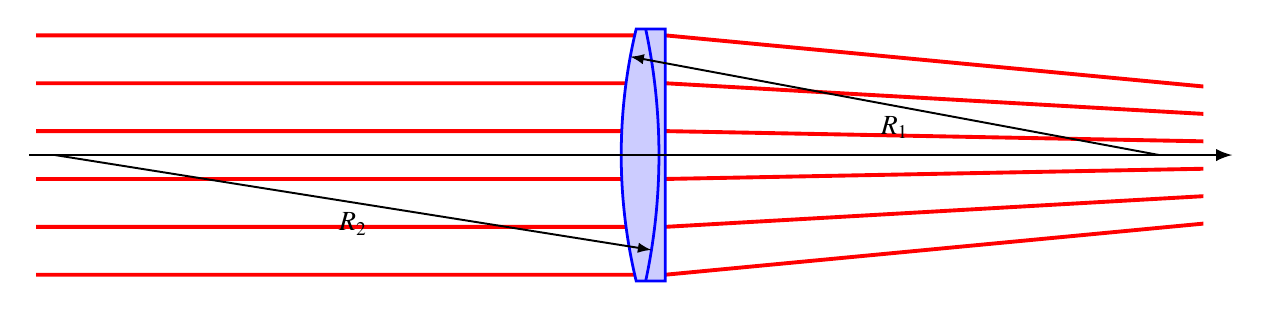
\begin{tikzpicture}[>=latex,thick,scale=0.8]

\def\done{0.6}
\def\dtwo{0.1}
\def\Rone{8.5413}
\def\Rtwo{9.5892}

\def\h{2.0}

\pgfmathparse{\h/\Rone}
\xdef\x{\pgfmathresult}
\pgfmathparse{atan(\x/sqrt(1-\x*\x))}
\xdef\aone{\pgfmathresult}

\pgfmathparse{\h/\Rtwo}
\xdef\x{\pgfmathresult}
\pgfmathparse{atan(\x/sqrt(1-\x*\x))}
\xdef\atwo{\pgfmathresult}

\pgfmathparse{-\done-\dtwo+\Rone*(1-cos(\aone))}
\xdef\xone{\pgfmathresult}

\pgfmathparse{-\dtwo-\Rtwo*(1-cos(\atwo))}
\xdef\xtwo{\pgfmathresult}

\begin{scope}
\clip ({-\Rtwo-\dtwo-0.3},-2) rectangle ({\Rone},2);
\foreach \y in {5,3,1,-1,-3,-5}{
\draw[color=red,line width=1.4pt] ({-\Rtwo-\done-\dtwo},{1.9*\y/5})--(0,{1.9*\y/5})--(20,0);
}
\end{scope}

\fill[color=blue!20]
	({\xone},{\h}) arc (180-\aone:180+\aone:\Rone)
	-- (0,{-\h})--(0,{\h})--cycle;

\draw[color=blue,line width=1pt]
	({\xone},{\h}) arc (180-\aone:180+\aone:\Rone)
	-- (0,{-\h})--(0,{\h})--cycle;

\draw[color=blue,line width=1pt]
	({\xtwo},{\h}) arc (\atwo:{-\atwo}:\Rtwo);

\draw[->,line width=0.7pt] ({\Rone-\done-\dtwo},0)
	--
	({\Rone-\done-\dtwo-\Rone*cos(\aone-3)},{\Rone*sin(\aone-3)});

\node at ({\Rone-\done-\dtwo-\Rone*cos(\aone-3)/2},{\Rone*sin(\aone-3)/2})
	[below] {$R_1$};

\draw[->,line width=0.7pt] ({-\dtwo-\Rtwo},0)
	--
	({-\dtwo-\Rtwo+\Rtwo*cos(-\atwo+3)},{\Rtwo*sin(-\atwo+3)});

\node at ({-\dtwo-\Rtwo+\Rtwo*cos(-\atwo+3)/2},{(\Rtwo*sin(-\atwo+3))/2})
	[below] {$R_2$};

\draw[->,line width=1.0pt] (-10.1,0)--(9,0);

\punkt{(\Rone-\done-\dtwo,0)}
\punkt{(-\dtwo-\Rtwo,0)}

\end{tikzpicture}

\end{document}

